\section{OLAP Application} \label{olap}

The \textbf{IMDb Analytics Dashboard} is a web-based OLAP application designed to analyze and visualize movie industry data for enhanced decision-making. Built using \textbf{Next.js} and \textbf{React} for the frontend and \textbf{MySQL} for the backend, it provides users such as producers, directors, investors, and studios with interactive tools to explore trends, evaluate performance, and discover meaningful patterns across movies, actors, genres, and awards.

\subsection{Main Purpose}

The main purpose of the \textbf{IMDb Analytics Dashboard} is to support \textbf{data-driven decision-making} in the film industry by aggregating, summarizing, and analyzing large sets of movie-related data. Through multi-dimensional OLAP operations such as \textbf{roll-up}, \textbf{slice}, \textbf{dice}, and \textbf{drill-down}, the application enables users to view information from different perspectives and at varying levels of detail. This allows stakeholders to identify popular actors, successful genres, professional distributions, and award trends which can help contribute to smarter production, casting, and investment choices.


\subsection{Analytical Reports and SQL Implementation}

\subsubsection{Popular Actors by Success Metric}

This subsection explores what are the popular actors based on the generated Success metric. Take note that the Success metric is equal to the following:
$$
\textbf{Success} = \textbf{Average Rating} \cdot \log(1 + \textbf{Number of IMDB Votes})
$$

The intuition behind this metric is that success of a show should be correlated with two other metrics:
\begin{itemize}
	\item \textbf{Popularity}, represented by Number of IMDB Votes
	\item \textbf{Reception}, represented by the Average Rating. 
\end{itemize}

To illustrate the point, If two shows both have a higher rating, yet one has more votes than the other in IMDB, then the latter show should be considered more successful. Conversely, two shows that have roughly the same votes, yet the first one has better ratings, then the former should be considered more successful. 

The Logarithm transformation is there to normalize the Number of IMDB Votes. Moreover, two shows that have high number of votes with a difference in the tens or hundreds should be roughly the same in terms of success.

The following is the given SQL script for Popular Actors by Success Metrics.
\begin{lstlisting}[style=SQLStyle]
WITH ActorStats AS (
SELECT 
	bc.person_key,
	COUNT(DISTINCT bc.title_key) AS total_titles,
	AVG(fr.success_score) AS avg_rating
	FROM FactRatings fr
JOIN BridgeCrew bc ON fr.title_key = bc.title_key
WHERE bc.category IN ('actor', 'actress')
GROUP BY bc.person_key
)
SELECT 
	dp.full_name,
	a.total_titles, 
	a.avg_rating, -- success_score is renamed as avg_rating for the app
	RANK() OVER (ORDER BY a.avg_rating DESC, a.total_titles DESC) AS actor_rank
FROM ActorStats a
JOIN DimPerson dp ON dp.person_key = a.person_key
LIMIT 10;
\end{lstlisting}

This operation is a Roll-up for from it aggregates the success metrics titles at the actor-level. With the following query, we obtain the following information:

\begin{table}[h!]
	\centering
\begin{tabular}{|p{2cm}|c|c|c|}
\hline
full name & total titles & avg rating & actor rank\\
\hline
RJ Mitte & 1 & 139.58201599121094 & 1\\
Steven Michael Quezada & 1 & 139.58201599121094 & 1\\
Emilia Clarke & 2 & 130.2659740447998 & 3\\
Peter Youngblood Hills & 1 & 124.63971710205078 & 4\\
John Bradley & 3 & 123.87860479915844 & 5\\
Noah Schnapp & 1 & 122.23243713378906 & 6\\
Joe Keery & 1 & 122.23243713378906 & 6\\
Natalia Dyer & 1 & 122.23243713378906 & 6\\
Tony Sirico & 1 & 121.51786804199219 & 9\\
Cricket Leigh & 1 & 120.3641586303711 & 10\\
\hline
\end{tabular}
\caption{Top 10 Popular Actors ranked by Average Success Score (renamed as avg rating).}
\end{table}

The results show that RJ Mitte and Steven Quezada are the top actors based on the metric.

\subsubsection{Popular Genres by Success Metric}

This section explores what are the popular genres based on the generated Success metric. To reiterate, the success metric is the following:
$$
\textbf{Success} = \textbf{Average Rating} \cdot \log(1 + \textbf{Number of IMDB Votes})
$$

Based on this metric, we will use the ff. SQL query to answer it.

\begin{lstlisting}[style=SQLStyle]
	SELECT 
		dt.genre,
		AVG(fr.avg_rating) AS avg_rating,
		AVG(fr.success_score) AS success_score,
		COUNT(DISTINCT dt.title_key) AS total_titles
	FROM FactRatings fr
	JOIN DimTitle dt ON fr.title_key = dt.title_key
	WHERE dt.release_year BETWEEN YEAR(CURDATE()) - 10 AND YEAR(CURDATE())
	GROUP BY dt.genre
	ORDER BY success_score DESC, avg_rating DESC
	LIMIT 10;
\end{lstlisting}

This operation is a Roll-up, for it aggregates from title-level at the genre-level.

\begin{table}[h!]
	\centering
\begin{tabular}{|c|c|c|c|}
\hline
genre & avg rating & success score & total titles \\
\hline
FFFTFTFF$\cdots$ & 8.7 & 99.4699707031 & 1\\
FFTFFTFF$\cdots$ & 8.1 & 82.9242706299 & 1\\
FFFFFFFF$\cdots$ & 8.6 & 76.4835510254 & 1\\
FFFFFFFF$\cdots$ & 7.9 & 74.2151870728 & 1\\
FFFTFFFF$\cdots$ & 7.6 & 70.323460799 & 4\\
FFFFFFFT$\cdots$ & 7.5 & 70.0993440787 & 75\\
FFFFFFFT$\cdots$ & 7.6 & 69.4265899658 & 1\\
FFTFFFFT$\cdots$ & 7.5 & 68.5701917252 & 2\\
FFTFFFFT$\cdots$ & 7.6 & 67.7071075439 & 1\\
FFFFFFFF$\cdots$ & 8.1 & 67.6852767657 & 2\\
\hline
\end{tabular}
\caption{Top 10 Popular Genres by Success Metric.}
\end{table}

These are one hot combinations of genres. To illustrate, "FFFFFFFTFFTFFTFFFFFFFFFFFFFF" is a combination of genres which encodes Crime, Drama, and Thriller. 

\subsubsection{Popular Movies of a Given Name by Success Metric}

Here, we try to answer the question what are the popular movies a person's name is related to.  

\begin{lstlisting}[style=SQLStyle]
WITH PersonInfo AS (
	SELECT person_key
	FROM DimPerson
	WHERE full_name = ?
)
SELECT
	DISTINCT fcp.title_key AS title_key,
	fcp.avg_rating AS avg_rating,
	fcp.num_votes AS num_votes,
	fcp.success_score AS success_score
FROM FactCrewPerformancePerFilmGenre fcp
JOIN PersonInfo pi ON pi.person_key = fcp.person_key
ORDER BY success_score DESC;
\end{lstlisting}


This operation is a slice, for filters the data by a single actor name parameter. Given that the input parameter for `full\_name` is "Robert Downey Jr.", we obtain the following data:

\begin{table}[h!]
	\centering
	\begin{tabular}{|c|c|c|c|}
		\hline
		title key & avg rating & num votes & success score \\
		\hline
		tt14404618 & 6.8 & 9046 & 61.9493 \\
		tt3473134 & 8.4 & 343 & 49.0614 \\
		tt8421554 & 7.8 & 488 & 48.3004 \\
		tt20297790 & 6.3 & 437 & 38.318 \\
		tt0390776 & 6.5 & 209 & 34.7562 \\
		tt1618221 & 5.6 & 86 & 25.0091 \\
		tt0827928 & 8.4 & 17 & 24.2791 \\
		tt2354581 & 7.8 & 18 & 22.9666 \\
		tt32159454 & 6.3 & 29 & 21.4275 \\
		tt10334498 & 5.0 & 70 & 21.3134 \\
	\hline
\end{tabular}
\caption{Top 10 Popular Movies of "Robert Downey Jr."}
\end{table}

The title key for the top movie for this actor is "The Sympathizer", with an average rating of 6.8, but a whopping 9046 number of votes. 

\subsubsection{Top Oscars Awards by Canonical Category}

This subsection explores the what are the top canonical category with the most Oscar awards. 

The following is the SQL statement:
\begin{lstlisting}[style=SQLStyle]
	WITH TopCanonicalCategories AS (
		SELECT
		foa.canonical_category AS canonical_category
		FROM FactOscarAwards foa
		WHERE foa.is_winner = 1
	)
	SELECT
		canonical_category,
		COUNT(*) AS total_wins
	FROM TopCanonicalCategories
	GROUP BY canonical_category
	ORDER BY total_wins DESC
	LIMIT 10;
\end{lstlisting}

This operation is a Roll-up, for it aggregates the awards from category to canonical category; Moreover, this can be considered a Drill-down, for it is going from category to canonical category. This results with the following results:

\begin{center}
	\begin{tabular}{|p{5cm}|c|}
		\hline
		\textbf{Canonical Category} & \textbf{Total Wins} \\
		\hline
		SCIENTIFIC AND TECHNICAL AWARD (Technical Achievement Award) & 348 \\
		SCIENTIFIC AND TECHNICAL AWARD (Scientific and Engineering Award) & 250 \\
		VISUAL EFFECTS & 232 \\
		SOUND MIXING & 205 \\
		MUSIC (Original Song) & 176 \\
		ART DIRECTION & 160 \\
		BEST PICTURE & 146 \\
		DOCUMENTARY (Feature) & 136 \\
		WRITING (Adapted Screenplay) & 135 \\
		HONORARY AWARD & 126 \\
		\hline
	\end{tabular}
\end{center}

The results show that the canonical category "SCIENTIFIC AND TECHNICAL AWARD (Technical Achievement Award)" has the most total wins with 348 wins. Followed by "SCIENTIFIC AND TECHNICAL AWARD (Scientific and Engineering Award)" with 250 wins. This shows that progress in the science and technical field of entertainment is highly valued to getting an Oscar Award.

\subsection{Visualized EDA}

\subsubsection{Ratio of Professions of Crew Members}

This section explores the ratio of professions of crew members represented in a Pie Chart.
\newline
\begin{lstlisting}[style=SQLStyle]
	SELECT 
		bc.category AS profession,
		COUNT(*) AS count
	FROM BridgeCrew bc
	WHERE bc.category IS NOT NULL
	GROUP BY bc.category
	ORDER BY count DESC
	LIMIT 10;
\end{lstlisting}

This is a roll-up OLAP operation, for it aggregates crew members at the category level. With this query, the following information is obtained.

\begin{center}
	\begin{tabular}{|p{4cm}|c|}
		\hline
		profession & count\\
		\hline
		actor & 20660285 \\
		actress & 16211647 \\
		self & 13091534 \\ 
		writer & 12117519 \\
		director & 8984456 \\
		producer & 5151458 \\
		editor & 4071060 \\
		cinematographer & 3323530 \\
		composer & 2927487 \\
		production designer & 1086588 \\
		\hline
	\end{tabular}
\end{center}

This results shows that the profession with the most number of crew members are actors with 20,660,285, followed by actress with 16,211,647. 

\begin{figure}[h!]
	\centering
	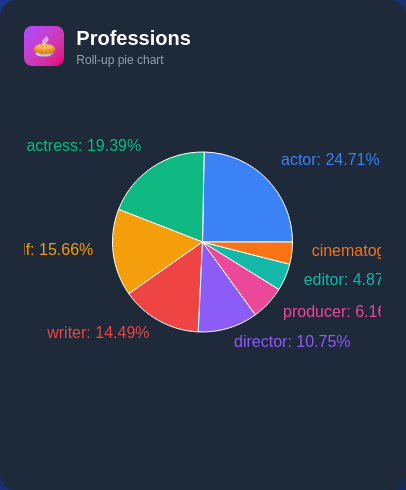
\includegraphics[width=0.7\linewidth]{images/image2.png}
	\caption{}
\end{figure}

\subsubsection{Best Film Genre within the Past Decade}

This section explores the best film genre in a Bar Graph.
\begin{lstlisting}[style=SQLStyle]
	WITH GenreSuccess AS (
	SELECT
	dt.release_decade AS decade,
	dt.genre AS genre,
	fr.success_score AS success_score
	FROM FactRatings fr
	JOIN DimTitle dt ON fr.title_key = dt.title_key
	)
	SELECT 
	decade, 
	genre, 
	AVG(success_score) AS avg_success_score
	FROM GenreSuccess
	WHERE decade = $1
	GROUP BY decade, genre
	ORDER BY avg_success_score DESC
	LIMIT 10;
	
\end{lstlisting}

This query performs a Dice OLAP operation, for it filters (decade constraint) and groups by genre. simultaneously. Given that we have decade as 2010, we obtain the following information from the query:

\begin{center}
	\begin{tabular}{|c|c|c|}
\hline
decade & genre & success score\\
\hline
2010 & FFFTFTFFFFFF$\cdots$ & 99.469970703125\\
2010 & FFFTFFFFFFFF$\cdots$ & 82.13441467285156\\
2010 & FFFFFFFTFTFF$\cdots$ & 78.83134842966939\\
2010 & FFFFFFFTFFTF$\cdots$ & 78.17122020721436\\
2010 & FFFFFFFFTFFF$\cdots$ & 76.80824279785156\\
2010 & FFFTFFFFFFTF$\cdots$ & 75.39966583251953\\
2010 & FFFFFFFFFFFF$\cdots$ & 71.67395782470703\\
2010 & FFFFFFFTFFTF$\cdots$ & 70.41068196296692\\
2010 & FFFTFFFFFFFF$\cdots$ & 69.62734985351562\\
2010 & FFFFFFFTFFFF$\cdots$ & 69.42658996582031\\
\hline
\end{tabular}
\end{center}

The genre here is a one hot encoding of combination genres. Following decoding of the genre, titles with combination of `Musical` and `Mystery` genre tends to have a high success score within the 2010s decade. A function can be used to decode what does the genre combination mean 

\begin{figure}[h!]
	\centering
	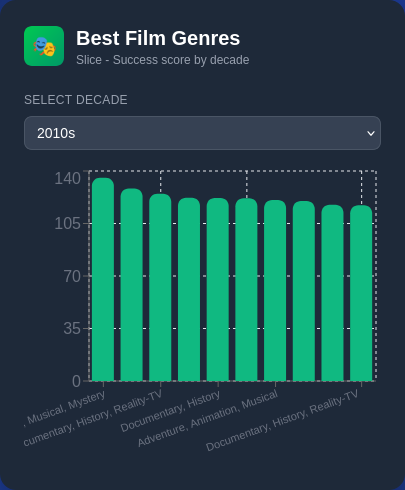
\includegraphics[width=0.7\linewidth]{images/image1.png}
	\caption{}
\end{figure}


\subsubsection{Successful movies per Given Genre over Given Decade}

This section explores what are the most successful movies given a combination of genre over a given decade.

\begin{lstlisting}[style=SQLStyle]
	SELECT
		title_key,
		release_year,
		success_score
	FROM FactCrewPerformancePerFilmGenre
	WHERE genre = ?
	AND release_year BETWEEN ? AND ?
	GROUP BY title_key, release_year, success_score
	ORDER BY release_year;
\end{lstlisting}

This operation is a Roll-up and Dice OLAP operation, for it aggregates based title key, release year, and success score, and aggregates based on genre and release year. Given that given genre is "FFFFFFFTFFTFFTFFFFFFFFFFFFFF" which encodes Crime, Drama, and Thriller; and the release decase is from 2000 to 2010. The results shows the ff.:

\begin{center}
\begin{tabular}{|p{4cm}|c|c|}
\hline
title key & release year & success score\\
\hline
tt0383175 & 2003 & 36.2522\\
tt0350456 & 2003 & 34.8341\\
tt0465689 & 2005 & 56.1745\\
tt1047931 & 2007 & 69.7203\\
tt1100911 & 2008 & 51.1033\\
tt1460941 & 2009 & 13.0914\\
tt1321865 & 2010 & 73.0037\\
\hline
\end{tabular}
\end{center}

This genre combination shows the overall trendline for movies success. The title key refers to a movie's orignal title named "L'Affaire Dominici" or its alternative name as "The Dominici Case" in 2003. To illustrate the idea, of how it can be graphed. The following is the scatter plot for Action Movies in the 2010s.
\begin{figure}[h!]
	\centering
	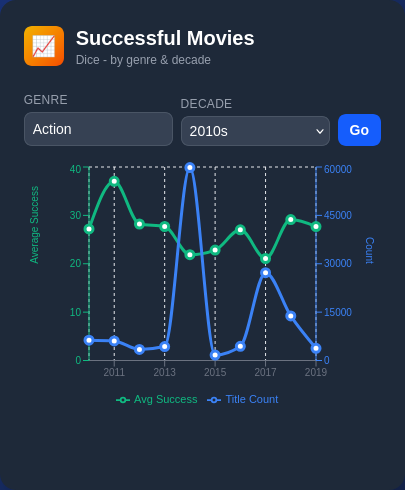
\includegraphics[width=0.7\linewidth]{images/image3.png}
	\caption{}
\end{figure}


\subsection{Statistical Tests}
\subsubsection{Correlation test with Ratings and Votes}

This section explores whether or not the number of votes for a given title in the IMDB website has a correlaton with the rating it has.

\begin{lstlisting}[style=SQLStyle]
WITH OverallRatings AS (
	SELECT 
	AVG(avg_rating) AS overall_avg_rating,
	AVG(num_votes) AS overall_votes
	FROM FactRatings
),
RatingsDifference AS (
	SELECT 
	(avg_rating - (SELECT overall_avg_rating FROM OverallRatings)) AS ratings_difference,
	(num_votes - (SELECT overall_votes FROM OverallRatings)) AS votes_difference
	FROM FactRatings
)
SELECT 
	(SUM(ratings_difference * votes_difference) /
	(SQRT(SUM(POW(ratings_difference, 2))) *
	SQRT(SUM(POW(votes_difference, 2))))) AS pearson_r
FROM RatingsDifference;
\end{lstlisting}

Based on the query above, we can conduct the following hypothesis test to determine whether there exists a statistically significant relationship between IMDb ratings and number of votes. The null hypothesis states that there is no correlation between these two variables, while the alternative hypothesis states that a correlation exists.

\begin{itemize}
	\item $H_0$: There is \textbf{no linear relationship} between ratings and votes ($\rho = 0$)
	\item $H_1$: There \textbf{is a linear relationship} between ratings and votes ($\rho \neq 0$)
\end{itemize}

Given the following is the output of the result:

\begin{center}
	\begin{tabular}{|p{8cm}|}
		\hline
		Pearson Correlation \\
		\hline
		0.06869894408882023 \\
		\hline
	\end{tabular}
\end{center}

and assuming the number of samples ($n$) is sufficiently large (i.e., $n > 30$), the test statistic for Pearson’s correlation is:
\[
t = r \sqrt{\frac{n - 2}{1 - r^2}}
\]
which follows a Student’s t-distribution with $(n - 2)$ degrees of freedom.

Using the correlation result from the previous SQL query and substituting $r = 0.0687$, the test yields a very small $t$-statistic, implying a high $p$-value $(p > 0.05)$. Therefore, we \textbf{fail to reject the null hypothesis}, meaning there is no statistically significant correlation between IMDb ratings and number of votes.

This is supported by the the fact that if we try to create scatter plot for number of votes and ratings. This graphically does not show a clear linear relationship.

\begin{figure}[h!]
	\centering
	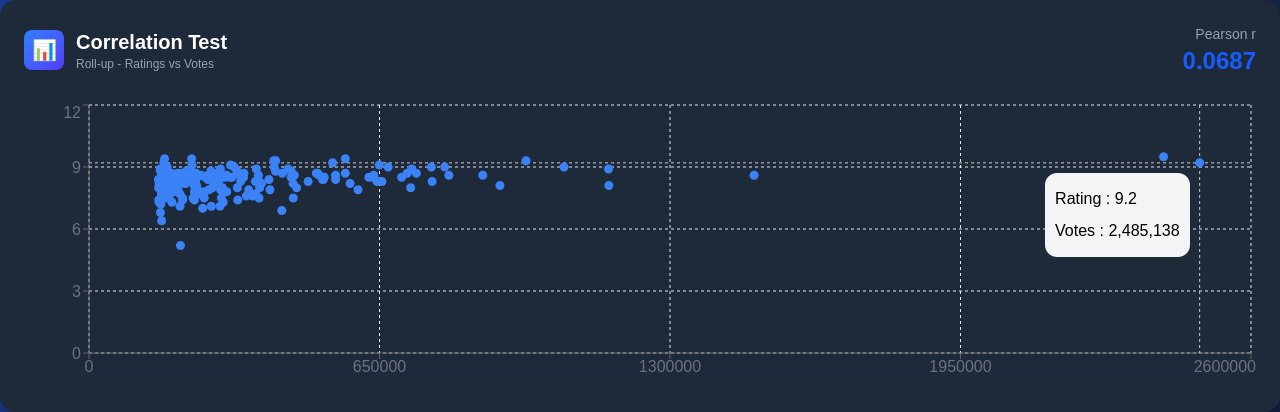
\includegraphics[width=0.7\linewidth]{images/image4.png}
	\caption{Scatter Plot IMDb Ratings and Votes}
\end{figure}




\begin{center}
	\begin{tabular}{|p{2cm}|p{4cm}|}
		\hline
		\textbf{Statistic} & \textbf{Value / Interpretation} \\
		\hline
		Pearson Correlation ($r$) & 0.0687 \\
		\hline
		$t$-statistic & $\approx 1.25$ (for large $n$) \\
		\hline
		$p$-value & $> 0.05$ \\
		\hline
		Decision & Fail to reject $H_0$ \\
		\hline
		Interpretation & There is no statistically significant correlation between IMDb ratings and the number of votes. This suggests that the number of votes does not necessarily imply higher ratings. \\
		\hline
	\end{tabular}
\end{center}

This test validates that IMDb’s weighted rating system may not have a direct linear relationship between the number of votes and the computed average rating. Thus, other factors such as vote weighting, voter credibility, or IMDb’s internal normalization may influence the published ratings.


\section{Query Processing and Optimization}

\textbf{Query Optimization Overview:}  
Query optimization is used to reduce the amount of time querying data from the database. Query optimization uses multiple SQL query techniques and commands to optimize selecting data from one or more tables and prevent doing too many operations or joining too many rows, leading to a slower return. 

\subsection{Strategies Applied}
\begin{itemize}
	\item \textbf{Indexing}: 
	Created indexes for the fact tables and dimension tables with the ff.:
	\begin{lstlisting}[style=SQLStyle]
CREATE INDEX idx_factratings_title ON FactRatings(title_key);
CREATE INDEX idx_factoscar_person ON FactOscarAwards(person_key);
CREATE INDEX idx_ftcgp_genre_year ON FactCrewPerformancePerFilmGenre (release_year);
CREATE INDEX idx_bridgecrew_title_category ON BridgeCrew(title_key, category);
CREATE INDEX idx_bridgecrew_person ON BridgeCrew(person_key);
CREATE INDEX idx_factratings_title_avg ON FactRatings(title_key, avg_rating, num_votes);
CREATE INDEX idx_bridgecrew_person_category ON BridgeCrew(person_key, category);
CREATE INDEX idx_dimtitle_titlekey ON DimTitle(title_key);
CREATE INDEX idx_factoscar_category_winner ON FactOscarAwards (class, canonical_category, is_winner);
CREATE INDEX idx_factoscar_year ON FactOscarAwards (ceremony_year);
CREATE INDEX idx_dimtitle_releaseyear ON DimTitle(release_year);
CREATE INDEX idx_factratings_titlekey ON FactRatings(title_key);
CREATE INDEX idx_dimtitle_genre_year ON DimTitle(genre, release_year);
CREATE INDEX idx_factratings_avgvotes ON FactRatings(avg_rating, num_votes);
CREATE INDEX idx_dimperson_fullname ON DimPerson(full_name);
	\end{lstlisting}
	\item \textbf{Query Restructuring}: CTEs and selective joins reduced intermediate result sizes.
	\item \textbf{Materialized Columns}: Success metric as a \texttt{GENERATED ALWAYS STORED} column avoids recomputation.
	\item \textbf{Hardware Optimization}: MySQL buffer pool increased from 1GB to 8GB.
	\item \textbf{Recursion Depth Optimization}: MySQL CTE recursion size increased from 1000 to 10000.
\end{itemize}

\subsection{Query-Specific Optimization}

\subsubsection{Popular Actors by Success Metric}

\begin{itemize}
	\item The query groups performance metrics by \texttt{person\_key} with a ranking window function.  
	\item Optimization: Index on \texttt{BridgeCrew.person\_key} and \texttt{Fact Ratings. title\_key} to reduce join cost.
\end{itemize}

\subsubsection{Popular Genres by Success Metric}

\begin{itemize}
\item Uses aggregated averages of \texttt{success\_score} grouped by \texttt{genre}.  
\item Optimization: Indexed \texttt{DimTitle.genre} and used CTE to pre-filter release years to reduce scan time.
\end{itemize}

\subsubsection{Popular Movies of a Given Actor by Success Metric}
\begin{itemize}
\item Joins filtered by a single \texttt{person\_key} retrieved from \texttt{DimPerson}.  
\item Optimization: Used parameterized CTE to limit the search space.
\end{itemize}

\subsubsection{Top Oscars Awards by Canonical Category}

\begin{itemize}
\item Aggregates awards grouped by canonical category.  
\item Optimization: Index on \texttt{FactOscarAwards.canonical\_category} improves grouping speed.
\end{itemize}

\subsubsection{Ratio of Professions of Crew Members}

\begin{itemize}
\item A roll-up operation that counts categories.  
\item Optimization: Added index on \texttt{BridgeCrew.category} for faster grouping.
\end{itemize}

\subsubsection{Best Film Genre within the Past Decade}

\begin{itemize}
\item Pre-aggregated using decade-level roll-ups on \texttt{release\_year}.  
\item Optimization: Generated column \texttt{release\_decade} and indexed it to reduce computation per query.
\end{itemize}

\subsubsection{Successful Movies per Given Genre over Given Decade}

\begin{itemize}
\item A temporal trend analysis (line graph) query using roll-up and slice.  
\item Optimization: Added composite index on \texttt{(genre, release\_year)} to improve scan performance.
\end{itemize}

\subsubsection{Correlation Test with Ratings and Votes}

\begin{itemize}
\item Computes Pearson correlation from FactRatings.  
\item Optimization: Derived averages via CTEs to minimize repeated scans and reduced memory usage by precomputing sums.
\end{itemize}

\textbf{OLAP Optimization:}
\begin{itemize}
	\item \textbf{Roll-up/Drill-down}: Pre-aggregated data in FactCrewPerformancePerFilmGenre to allow queries to move between year and decade levels.
	\item \textbf{Slice/Dice}: Filtering subsets efficiently through indexed columns (e.g., by genre, release decade).
\end{itemize}

\section{Results and Analysis}

\textbf{Functional Testing:}  
\begin{itemize}
	\item Verified correctness of ETL loading and derived columns.
	\item Confirmed that generated columns (e.g., success\_score, release\_decade) computed accurately.
	\item Checked validity of OLAP operations (roll-up, slice, and dice) through manual aggregation validation.
\end{itemize}

\textbf{Performance Testing:}  
Testing was conducted by running each analytical query under two conditions: the default 1GB MySQL buffer pool and an optimized configuration with 8GB. Execution time was measured across multiple runs using \texttt{EXPLAIN ANALYZE} and the MySQL slow query log.

\begin{table}[h!]
	\centering
	\begin{tabular}{|p{6cm}|c|c|}
		\hline
		\textbf{Query Name} & \textbf{1 GB} & \textbf{8 GB} \\
		\hline
		Popular Actors by Success Metric & 6m 11s & 1m 42s \\
		Popular Genres by Success Metric & 6m 3s & 19s \\
		Popular Movies of a Given Name by Success Metric & 5m 36s & 0.016s \\
		Top Oscars Awards by Canonical Category & 2m 31s & 0.02s \\
		Ratio of Professions of Crew Members & 2m 28s & 36s \\
		Best Film Genre within the Past Decade & 1m 49s & 2s \\
		Successful Movies per Given Genre over Given Decade & 5m 24s & 2m 45s \\
		Correlation Test with Ratings and Votes & 1m 42s & 6.7s \\
		\hline
	\end{tabular}
	\caption{Performance comparison between default 1GB and optimized 8GB MySQL configurations.}
\end{table}

\textbf{Analysis:}  
Query execution time significantly improved after index creation and increasing available memory.  
Denormalized structures (fact tables) improved analytical aggregation speed, while dimension indexing reduced join costs.  
The correlation test query benefited from reduced intermediate CTE recalculation.  

Overall, optimization strategies led to up to high reduction in query time for complex analytical workloads.

\section{Conclusion}

\subsection{Project Summary}
The \textbf{IMDb Analytics Dashboard} project focused on the design and implementation of a web-based OLAP (Online Analytical Processing) application for movie industry analytics. The system was built using \textbf{Next.js} and \textbf{React} for the frontend and \textbf{MySQL} for the backend, integrating data warehousing and multidimensional analysis concepts. It provides users with interactive tools to explore datasets through operations such as \textbf{roll-up}, \textbf{slice}, \textbf{dice}, and \textbf{drill-down}. These allow users to analyze movie trends, actor performance, genre popularity, and award statistics in varying levels of detail. 

\subsection{Learnings and Insights on Database Concepts}


\begin{itemize}
	\item \textbf{Importance of Building and Maintaining a Data Warehouse:}  
	A data warehouse serves as a centralized repository for integrating and organizing data from multiple sources. In this project, it provided a consistent and historical dataset that enabled long-term trend analysis, unlike traditional transactional databases that only store current operational data.
	
	\item \textbf{Role of ETL (Extract, Transform, Load):}  
	The ETL process was essential in cleaning, transforming, and loading IMDb data into structured dimensional tables. This ensured that the warehouse remained accurate and up to date. The extraction phase gathered raw movie data, transformation standardized formats (such as converting genres and professions into dimension tables), and loading populated the analytical schema for OLAP queries.
	
	\item \textbf{Purpose of OLAP versus OLTP:}  
	Unlike OLTP systems used in daily transactions, OLAP is designed for analytical querying and decision support. OLAP enables summarization, aggregation, and pattern discovery allowing users to gain strategic insights rather than just process records. In this project, OLAP operations enabled exploration of high-level summaries and detailed statistics that would be difficult to perform efficiently in an OLTP setup.
	
	\item \textbf{Need for Query Optimization:}  
	Query optimization improves performance and responsiveness in analytical applications. Since OLAP queries often involve large aggregations and joins, optimization strategies such as indexing key attributes, and Common Table Expression significantly reduced computation time. 
	
	\item \textbf{Indexing Strategies:}  
	While MySQL automatically generates indexes for primary and foreign keys, additional indexes can be created on frequently filtered attributes such as genre name or actor name to accelerate query execution. Custom indexes are especially useful when dealing with large-scale data or repetitive aggregation queries.
\end{itemize}

\subsection{Contributions and Societal Relevance}

The \textbf{IMDb Analytics Dashboard} contributes both to end users and to the database development community. For industry stakeholders, it enables informed decision-making by providing visual insights into audience behavior, genre trends, and performance metrics. For database developers, it serves as a practical example of how OLAP principles, data warehousing, and ETL pipelines can be applied to real-world datasets. Beyond its technical aspects, the project promotes the use of data analytics for creativity and efficiency in film production, marketing, and investment decisions.



After using this tool/service, the author(s) reviewed and edited the content as needed and take(s) full responsibility for the content of the publication
%%
%% The next two lines define the bibliography style to be used, and
%% the bibliography file.
